\documentclass[12pt,a4paper]{article}
\usepackage{amsmath, amssymb, geometry, booktabs, xcolor, hyperref,
            listings, pgfplots, tcolorbox, enumitem, fancyhdr, tikz, array}
\usepgfplotslibrary{fillbetween}
\geometry{margin=2.5cm}
\pgfplotsset{compat=1.18}
\tcbuselibrary{skins, breakable}

% Define custom environments
\newtcolorbox{curiositybox}[1]{colback=yellow!10, colframe=orange!80, title=#1, breakable}
\newtcolorbox{infobox}[1]{colback=blue!5, colframe=blue!60, title=#1, breakable}
\newtcolorbox{mistakebox}[1]{colback=red!5, colframe=red!60, title=#1, breakable}
\newtcolorbox{learnbox}[1]{colback=green!5, colframe=green!60, title=#1, breakable}

% Header and Footer
\pagestyle{fancy}
\fancyhf{}
\lhead{Characteristic Equation}
\rhead{Unit 2 -- LAC}
\cfoot{\thepage}

% Document Title Setup
\title{\textbf{Characteristic Equation} \\ \large Unit 2 -- Eigenvalues, Eigenvectors, Diagonalization and Quadratic Forms}
\author{Department of Mathematics}
\date{\today}

\begin{document}
\maketitle
\tableofcontents
\newpage

%============================================================
\section{Real-World Engineering Hook}
%============================================================

\begin{curiositybox}{Why Should an Engineer Care?}
Consider a feedback control system for an autonomous vehicle's lane-keeping mechanism.
The system's dynamics are encoded in a state matrix $A$, and the \emph{characteristic equation}
$\det(A - \lambda I) = 0$ determines every natural frequency and damping mode of that system.
When an engineer applies the \textbf{Routh--Hurwitz criterion}, they are directly interrogating
this polynomial: if any root has a non-negative real part, the vehicle will drift out of lane
rather than converge to it---a potentially fatal instability.

In mechanical vibration analysis, the same polynomial governs natural frequencies of a
multi-storey building during an earthquake. Engineers designing seismic isolation systems
must ensure that repeated roots (algebraic multiplicity $> 1$) do not arise at the driving
frequency, because repeated roots in the characteristic equation can produce resonance
behaviour that standard damping calculations underestimate.
Whether you are designing aircraft autopilots, power-grid regulators, or robotic joints,
computing the characteristic equation correctly is the gateway skill.
\end{curiositybox}

%============================================================
\section{Why This Topic Exists}
%============================================================

\begin{center}
\begin{tabular}{@{}p{4cm} p{5cm} p{5.5cm}@{}}
\toprule
\textbf{Atomic Sub-Topic} & \textbf{Core Mathematical Idea} & \textbf{Engineering Consequence} \\
\midrule
Characteristic Polynomial Definition
  & $p(\lambda)=\det(A-\lambda I)$, degree $n$
  & Encodes all stability information of a dynamic system; used directly in Laplace-domain analysis \\
\addlinespace
Roots as Eigenvalues
  & Roots of $p(\lambda)=0$ are eigenvalues; trace $=\sum\lambda_i$; det $=\prod\lambda_i$
  & Quick sanity checks: trace and determinant let engineers verify eigenvalue calculations without full re-computation \\
\addlinespace
Cofactor Expansion for $3\times3$
  & Systematic row/column expansion for $\det(A-\lambda I)$
  & Essential for hand calculation and symbolic derivation of transfer function denominators \\
\addlinespace
Shortcuts and Special Cases
  & Diagonal/triangular structure; eigenvalues of $A^2$, $A^{-1}$, $A^\top$
  & Saves computation time for sparse or structured system matrices common in finite element models \\
\addlinespace
Algebraic Multiplicity
  & Root multiplicity of $\lambda_0$ in $p(\lambda)$
  & Repeated eigenvalues signal potential non-diagonalizability; critical in modal analysis and Jordan form decomposition \\
\bottomrule
\end{tabular}
\end{center}

\vspace{1em}
\begin{learnbox}{Core Learning Objectives}
After studying this topic you will be able to:
\begin{itemize}[leftmargin=*]
  \item Write the characteristic polynomial $p(\lambda)=\det(A-\lambda I)$ for any $n\times n$ matrix.
  \item Use trace and determinant to verify eigenvalue sums and products.
  \item Perform cofactor expansion on $3\times 3$ matrices to obtain the cubic characteristic polynomial.
  \item Apply shortcuts for diagonal, triangular, and block-diagonal matrices.
  \item Compute eigenvalues of derived matrices ($A^2$, $A^{-1}$, $A^\top$) from the eigenvalues of $A$.
  \item Define and compute algebraic multiplicity and relate it to diagonalizability.
\end{itemize}
\end{learnbox}

%============================================================
\section{Intuition, Definitions, and Worked Examples}
%============================================================

% -------------------------------------------------------
\subsection{Characteristic Polynomial Definition}
% -------------------------------------------------------

When we subtract $\lambda$ times the identity from a matrix $A$ and take the determinant,
we get a polynomial in $\lambda$. This polynomial encodes the ``spectrum'' of $A$---every
eigenvalue is hidden inside it as a root. The degree of this polynomial equals the size of
the matrix, so a $2\times 2$ system produces a quadratic and a $3\times 3$ system produces
a cubic. The sign convention used here is $p(\lambda)=\det(A-\lambda I)$, which produces a
leading term $(-\lambda)^n$; some textbooks write $\det(\lambda I - A)$, yielding $+\lambda^n$.
Either convention gives the same roots.

\begin{infobox}{Characteristic Polynomial --- Formal Definition}
Let $A$ be an $n\times n$ real or complex matrix. The \textbf{characteristic polynomial} of $A$ is
\[
  p(\lambda) = \det(A - \lambda I_n).
\]
\textbf{Key properties:}
\begin{itemize}[leftmargin=*]
  \item $p(\lambda)$ is a polynomial of degree $n$ in $\lambda$.
  \item Leading coefficient: $(-1)^n$.
  \item Constant term: $p(0) = \det(A)$.
  \item The \textbf{characteristic equation} is $p(\lambda) = 0$.
  \item The roots of $p(\lambda)=0$ are precisely the eigenvalues of $A$.
\end{itemize}
\textbf{For a $2\times 2$ matrix:}
\[
  A = \begin{pmatrix} a & b \\ c & d \end{pmatrix}, \quad
  p(\lambda) = \det\begin{pmatrix} a-\lambda & b \\ c & d-\lambda \end{pmatrix}
             = (a-\lambda)(d-\lambda) - bc
             = \lambda^2 - (a+d)\lambda + (ad-bc).
\]
\end{infobox}

\textbf{Worked Example 1.1 --- Characteristic Polynomial of a $2\times 2$ Matrix}

Let
\[
  A = \begin{pmatrix} 5 & 3 \\ 2 & 4 \end{pmatrix}.
\]
Step 1: Form $A - \lambda I$:
\[
  A - \lambda I = \begin{pmatrix} 5-\lambda & 3 \\ 2 & 4-\lambda \end{pmatrix}.
\]
Step 2: Compute the determinant:
\[
  p(\lambda) = (5-\lambda)(4-\lambda) - (3)(2).
\]
Step 3: Expand $(5-\lambda)(4-\lambda)$:
\[
  (5-\lambda)(4-\lambda) = 20 - 5\lambda - 4\lambda + \lambda^2 = \lambda^2 - 9\lambda + 20.
\]
Step 4: Subtract $6$:
\[
  p(\lambda) = \lambda^2 - 9\lambda + 20 - 6 = \lambda^2 - 9\lambda + 14.
\]
So the characteristic polynomial is $p(\lambda) = \lambda^2 - 9\lambda + 14$.

% -------------------------------------------------------
\subsection{Roots as Eigenvalues}
% -------------------------------------------------------

Once you have $p(\lambda)$, solving $p(\lambda)=0$ gives you all eigenvalues.
Two elegant shortcuts exist that do \emph{not} require solving the polynomial from scratch:
the \textbf{trace} (sum of diagonal entries) equals the sum of all eigenvalues, and the
\textbf{determinant} equals the product of all eigenvalues.
These relations act as built-in verification tools---if your computed eigenvalues do not
sum to the trace or multiply to the determinant, you made an arithmetic error somewhere.

\begin{infobox}{Roots and Trace--Determinant Relations}
Let $\lambda_1, \lambda_2, \ldots, \lambda_n$ be the eigenvalues of $A$ (counted with multiplicity). Then:
\[
  \sum_{i=1}^{n} \lambda_i = \operatorname{tr}(A) = \sum_{i=1}^{n} a_{ii},
\]
\[
  \prod_{i=1}^{n} \lambda_i = \det(A).
\]
For a $2\times 2$ matrix with $p(\lambda) = \lambda^2 - (\operatorname{tr}\, A)\lambda + \det(A)$:
\[
  \lambda_{1,2} = \frac{\operatorname{tr}(A) \pm \sqrt{(\operatorname{tr}\,A)^2 - 4\det(A)}}{2}.
\]
\end{infobox}

\textbf{Worked Example 2.1 --- Finding Eigenvalues and Verifying Trace/Det}

Continue with $A = \begin{pmatrix} 5 & 3 \\ 2 & 4 \end{pmatrix}$ and $p(\lambda) = \lambda^2 - 9\lambda + 14$.

Step 1: Solve $\lambda^2 - 9\lambda + 14 = 0$ by factoring:
\[
  (\lambda - 7)(\lambda - 2) = 0 \implies \lambda_1 = 7,\quad \lambda_2 = 2.
\]
Step 2: Verify using trace:
\[
  \operatorname{tr}(A) = 5 + 4 = 9 = \lambda_1 + \lambda_2 = 7 + 2 = 9. \quad \checkmark
\]
Step 3: Verify using determinant:
\[
  \det(A) = (5)(4) - (3)(2) = 20 - 6 = 14 = \lambda_1 \cdot \lambda_2 = 7 \times 2 = 14. \quad \checkmark
\]
Both relations hold, confirming the eigenvalues are correct.

% -------------------------------------------------------
\subsection{Cofactor Expansion for \texorpdfstring{$3\times3$}{3x3} Matrices}
% -------------------------------------------------------

For a $3\times 3$ matrix, computing $\det(A-\lambda I)$ requires expanding a $3\times 3$
determinant whose entries are polynomials in $\lambda$. The cofactor expansion along the
first row is the most systematic approach. Each $2\times 2$ minor determinant will itself
contain $\lambda$ terms, so careful bookkeeping is essential. The result is always a cubic
polynomial $-\lambda^3 + c_2\lambda^2 + c_1\lambda + c_0$.

\begin{infobox}{Cofactor Expansion for $3\times3$ Characteristic Polynomial}
For $B = A - \lambda I$ with $B_{ij}$ denoting entries, expand along row 1:
\[
  \det(B) = B_{11}(B_{22}B_{33}-B_{23}B_{32})
           - B_{12}(B_{21}B_{33}-B_{23}B_{31})
           + B_{13}(B_{21}B_{32}-B_{22}B_{31}).
\]
Each $B_{ij} = a_{ij} - \lambda\delta_{ij}$, so diagonal entries contain $\lambda$ and
off-diagonal entries are constants.

The resulting characteristic polynomial has the form:
\[
  p(\lambda) = -\lambda^3 + (\operatorname{tr}\,A)\lambda^2 - \frac{1}{2}\bigl[(\operatorname{tr}\,A)^2 - \operatorname{tr}(A^2)\bigr]\lambda + \det(A).
\]
\end{infobox}

\textbf{Worked Example 3.1 --- Full Cofactor Expansion on a $3\times3$ Matrix}

Let
\[
  A = \begin{pmatrix} 2 & 1 & 0 \\ 1 & 3 & 1 \\ 0 & 1 & 2 \end{pmatrix}.
\]
Step 1: Form $A - \lambda I$:
\[
  A - \lambda I = \begin{pmatrix} 2-\lambda & 1 & 0 \\ 1 & 3-\lambda & 1 \\ 0 & 1 & 2-\lambda \end{pmatrix}.
\]
Step 2: Expand $\det(A-\lambda I)$ along row 1. The $(1,3)$ entry is $0$, so only two cofactors contribute:
\[
  p(\lambda) = (2-\lambda)\det\begin{pmatrix} 3-\lambda & 1 \\ 1 & 2-\lambda \end{pmatrix}
             - (1)\det\begin{pmatrix} 1 & 1 \\ 0 & 2-\lambda \end{pmatrix}.
\]
Step 3: Evaluate the $2\times 2$ minors:
\[
  M_1 = (3-\lambda)(2-\lambda) - (1)(1) = 6 - 3\lambda - 2\lambda + \lambda^2 - 1 = \lambda^2 - 5\lambda + 5.
\]
\[
  M_2 = (1)(2-\lambda) - (1)(0) = 2 - \lambda.
\]
Step 4: Assemble:
\[
  p(\lambda) = (2-\lambda)(\lambda^2 - 5\lambda + 5) - (2-\lambda).
\]
Step 5: Factor out $(2-\lambda)$:
\[
  p(\lambda) = (2-\lambda)\bigl[(\lambda^2 - 5\lambda + 5) - 1\bigr] = (2-\lambda)(\lambda^2 - 5\lambda + 4).
\]
Step 6: Factor the quadratic: $\lambda^2 - 5\lambda + 4 = (\lambda-1)(\lambda-4)$.
\[
  p(\lambda) = (2-\lambda)(\lambda-1)(\lambda-4).
\]
Eigenvalues: $\lambda_1 = 2$, $\lambda_2 = 1$, $\lambda_3 = 4$.

Step 7: Verify trace: $\operatorname{tr}(A)=2+3+2=7=2+1+4$. $\checkmark$

Step 8: Verify determinant:
$\det(A) = 2(6-1) - 1(2-0) = 10 - 2 = 8 = 2\times1\times4$. $\checkmark$

% -------------------------------------------------------
\subsection{Shortcuts and Special Cases}
% -------------------------------------------------------

Many matrices that arise in engineering applications have special structure---diagonal,
triangular, or block-diagonal---that allows reading off eigenvalues directly without
computing any determinant. Additionally, if you know the eigenvalues of $A$, you can
immediately state the eigenvalues of $A^2$, $A^{-1}$, and $A^\top$ without any extra work.

\begin{infobox}{Shortcuts for Structured Matrices and Derived Eigenvalues}
\textbf{Diagonal matrix} $D = \operatorname{diag}(d_1,d_2,\ldots,d_n)$:
$\quad \det(D-\lambda I) = \prod_{i=1}^n(d_i-\lambda)$, so eigenvalues are $d_1,d_2,\ldots,d_n$.

\textbf{Upper (or lower) triangular matrix:}
Eigenvalues are the diagonal entries $a_{11},a_{22},\ldots,a_{nn}$.

\textbf{Block-diagonal matrix} $B = \operatorname{diag}(B_1,B_2)$:
$p(\lambda) = p_{B_1}(\lambda)\cdot p_{B_2}(\lambda)$.

\textbf{Eigenvalues of derived matrices} (if $\lambda$ is an eigenvalue of $A$):
\begin{itemize}[leftmargin=*]
  \item $A^k$ has eigenvalue $\lambda^k$ (for any positive integer $k$).
  \item $A^{-1}$ (if it exists) has eigenvalue $1/\lambda$.
  \item $A^\top$ has the same eigenvalues as $A$ (since $\det(A^\top - \lambda I) = \det(A-\lambda I)$).
  \item $A + cI$ has eigenvalue $\lambda + c$ for any scalar $c$.
\end{itemize}
\end{infobox}

\textbf{Worked Example 4.1 --- Shortcuts in Action}

Let
\[
  A = \begin{pmatrix} 3 & 0 & 0 \\ 0 & -1 & 0 \\ 0 & 0 & 5 \end{pmatrix}.
\]
Since $A$ is diagonal, eigenvalues are immediately $\lambda_1=3$, $\lambda_2=-1$, $\lambda_3=5$.

Now find the eigenvalues of $A^2$:
\[
  A^2 = \begin{pmatrix} 9 & 0 & 0 \\ 0 & 1 & 0 \\ 0 & 0 & 25 \end{pmatrix},
  \quad \text{eigenvalues } 3^2=9,\; (-1)^2=1,\; 5^2=25. \quad \checkmark
\]
Find eigenvalues of $A^{-1}$: $A^{-1}=\operatorname{diag}(1/3,-1,1/5)$, eigenvalues $1/3,-1,1/5$.
Verify: $1/\lambda_1 = 1/3$, $1/\lambda_2 = 1/(-1) = -1$, $1/\lambda_3=1/5$. $\checkmark$

Since $A$ is diagonal (hence symmetric), $A^\top = A$ trivially has the same eigenvalues.

% -------------------------------------------------------
\subsection{Algebraic Multiplicity}
% -------------------------------------------------------

The characteristic polynomial $p(\lambda)$ can have repeated roots. When a root $\lambda_0$
appears $k$ times in the factored form of $p(\lambda)$, we say its \textbf{algebraic multiplicity}
is $k$. This is a purely polynomial concept---it simply counts how many times a root is
``used up'' in the factorisation. High algebraic multiplicity does not automatically imply
that the corresponding eigenspace is large; that is a separate question answered by
\textbf{geometric multiplicity}. The interplay between these two numbers determines
whether $A$ is diagonalizable.

\begin{infobox}{Algebraic Multiplicity --- Definition and Properties}
Let $\lambda_0$ be a root of $p(\lambda)=\det(A-\lambda I)$. The \textbf{algebraic multiplicity} of
$\lambda_0$ is the largest integer $m$ such that $(\lambda - \lambda_0)^m$ divides $p(\lambda)$.

\textbf{Key facts:}
\begin{itemize}[leftmargin=*]
  \item $\sum_i m_i = n$ (total multiplicity equals matrix size).
  \item Algebraic multiplicity $m \geq$ geometric multiplicity $g \geq 1$.
  \item $A$ is diagonalizable if and only if $m_i = g_i$ for every eigenvalue $\lambda_i$.
  \item Repeated eigenvalues ($m > 1$) do \emph{not} guarantee non-diagonalizability;
        check geometric multiplicity separately.
\end{itemize}
\end{infobox}

\textbf{Worked Example 5.1 --- Repeated Eigenvalue and Algebraic Multiplicity}

Let
\[
  B = \begin{pmatrix} 4 & 1 & 0 \\ 0 & 4 & 1 \\ 0 & 0 & 6 \end{pmatrix}.
\]
$B$ is upper triangular, so eigenvalues are the diagonal entries: $4, 4, 6$.

Step 1: Write the characteristic polynomial:
\[
  p(\lambda) = (4-\lambda)^2(6-\lambda).
\]
Step 2: Identify multiplicities:
\begin{itemize}[leftmargin=*]
  \item $\lambda_1 = 4$: algebraic multiplicity $m_1 = 2$.
  \item $\lambda_2 = 6$: algebraic multiplicity $m_2 = 1$.
  \item Total: $2 + 1 = 3 = n$. $\checkmark$
\end{itemize}
Step 3: Check diagonalizability for $\lambda=4$. Compute $B-4I$:
\[
  B - 4I = \begin{pmatrix} 0 & 1 & 0 \\ 0 & 0 & 1 \\ 0 & 0 & 2 \end{pmatrix}.
\]
$\operatorname{rank}(B-4I) = 2$, so $\dim(\ker(B-4I)) = 3-2 = 1 = g_1$.
Since $m_1=2 > g_1=1$, the matrix $B$ is \textbf{not diagonalizable}.

%============================================================
\section{Visual Artifacts and Geometric Interpretation}
%============================================================

\subsection*{4.1 Plot of a Cubic Characteristic Polynomial}

The following plot shows the cubic polynomial
$p(\lambda) = -((\lambda-1)(\lambda-3)(\lambda-5)) = -\lambda^3+9\lambda^2-23\lambda+15$
with roots marked on the $\lambda$-axis.

\begin{center}
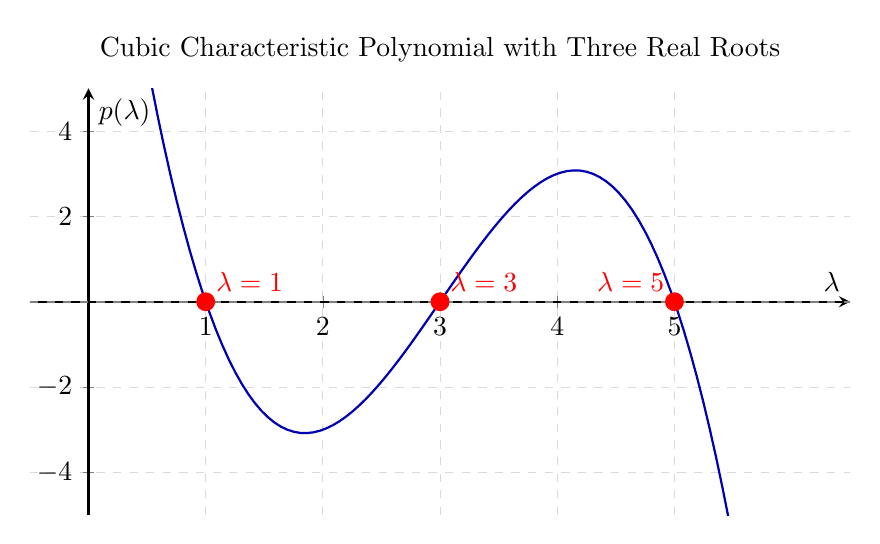
\begin{tikzpicture}
\begin{axis}[
  width=12cm, height=7cm,
  xlabel={$\lambda$},
  ylabel={$p(\lambda)$},
  title={Cubic Characteristic Polynomial with Three Real Roots},
  xmin=-0.5, xmax=6.5,
  ymin=-5, ymax=5,
  xtick={1,2,3,4,5},
  grid=major,
  grid style={dashed, gray!30},
  axis lines=center,
  samples=120,
  domain=-0.3:6.3,
  thick
]
\addplot[blue!70!black, thick] {-x^3 + 9*x^2 - 23*x + 15};
\addplot[only marks, mark=*, mark size=3pt, red] coordinates {(1,0) (3,0) (5,0)};
\node[above right, red] at (axis cs:1,0) {$\lambda=1$};
\node[above right, red] at (axis cs:3,0) {$\lambda=3$};
\node[above left, red] at (axis cs:5,0) {$\lambda=5$};
\addplot[dashed, gray] coordinates {(-0.5,0)(6.5,0)};
\end{axis}
\end{tikzpicture}
\end{center}

\subsection*{4.2 Trace and Determinant as Eigenvalue Invariants}

For a $2\times 2$ matrix, the trace equals the sum of eigenvalues and the determinant equals
their product. The diagram below illustrates this for a matrix with eigenvalues $\lambda_1$ and $\lambda_2$.

\begin{center}
\begin{tikzpicture}[
  node distance=1.8cm,
  box/.style={rectangle, draw, rounded corners, minimum width=3.5cm, minimum height=1cm, align=center},
  arrow/.style={->, thick, >=stealth}
]
\node[box, fill=blue!10] (mat) {Matrix $A = \begin{pmatrix} a & b \\ c & d \end{pmatrix}$};
\node[box, fill=orange!15, below left=1.5cm and 1cm of mat] (trace) {$\operatorname{tr}(A) = a+d$};
\node[box, fill=green!15, below right=1.5cm and 1cm of mat] (det) {$\det(A) = ad-bc$};
\node[box, fill=yellow!20, below=3.2cm of mat] (eig) {$\lambda_1 + \lambda_2 = \operatorname{tr}(A)$ \\ $\lambda_1 \cdot \lambda_2 = \det(A)$};
\draw[arrow] (mat) -- (trace) node[midway, left]{sum of diag};
\draw[arrow] (mat) -- (det) node[midway, right]{product rule};
\draw[arrow] (trace) -- (eig);
\draw[arrow] (det) -- (eig);
\end{tikzpicture}
\end{center}

%============================================================
\section{Step-by-Step Algorithmic Workflow}
%============================================================

\begin{learnbox}{Algorithm: Characteristic Polynomial and Eigenvalues}
\textbf{For a $2\times 2$ matrix $A = \begin{pmatrix} a & b \\ c & d \end{pmatrix}$:}
\begin{enumerate}[leftmargin=*, label=\textbf{Step \arabic*.}]
  \item Form $A - \lambda I = \begin{pmatrix} a-\lambda & b \\ c & d-\lambda \end{pmatrix}$.
  \item Compute $p(\lambda) = (a-\lambda)(d-\lambda) - bc = \lambda^2 - (a+d)\lambda + (ad-bc)$.
  \item Set $p(\lambda) = 0$ and solve the quadratic: $\lambda = \frac{(a+d) \pm \sqrt{(a+d)^2 - 4(ad-bc)}}{2}$.
  \item Verify: $\lambda_1 + \lambda_2 = \operatorname{tr}(A)$ and $\lambda_1\lambda_2 = \det(A)$.
\end{enumerate}

\textbf{For a $3\times 3$ matrix:}
\begin{enumerate}[leftmargin=*, label=\textbf{Step \arabic*.}]
  \item Form $A - \lambda I$ (a $3\times 3$ matrix with $\lambda$ on the diagonal).
  \item Choose the row or column with the most zeros for expansion.
  \item For each chosen entry $B_{1j}$, compute the $2\times 2$ minor $M_{1j}$ and cofactor $C_{1j} = (-1)^{1+j}M_{1j}$.
  \item Expand: $p(\lambda) = \sum_j B_{1j} C_{1j}$.
  \item Collect like powers of $\lambda$ to write $p(\lambda) = -\lambda^3 + c_2\lambda^2 + c_1\lambda + c_0$.
  \item Verify: $c_2 = \operatorname{tr}(A)$, $c_0 = \det(A)$.
  \item Solve $p(\lambda) = 0$ by inspection, rational root theorem, or numerical methods.
  \item Identify algebraic multiplicity of each root.
\end{enumerate}
\end{learnbox}

%============================================================
\section{Fully Worked Step-by-Step Numerical Examples}
%============================================================

\subsection*{Example 1: $2\times 2$ Matrix --- Characteristic Polynomial, Eigenvalues, Verification}

Let
\[
  A = \begin{pmatrix} 7 & -2 \\ 3 & 2 \end{pmatrix}.
\]
\textbf{Step 1.} $\operatorname{tr}(A) = 7+2 = 9$, $\det(A) = (7)(2)-(-2)(3) = 14+6 = 20$.

\textbf{Step 2.} Characteristic polynomial:
\[
  p(\lambda) = \lambda^2 - 9\lambda + 20.
\]
\textbf{Step 3.} Solve $\lambda^2 - 9\lambda + 20 = 0$: discriminant $= 81 - 80 = 1$.
\[
  \lambda = \frac{9 \pm 1}{2} \implies \lambda_1 = 5,\quad \lambda_2 = 4.
\]
\textbf{Step 4.} Verify trace: $5+4=9$. $\checkmark$ \quad Verify det: $5\times4=20$. $\checkmark$

\subsection*{Example 2: $3\times 3$ Matrix --- Cofactor Expansion to Cubic Polynomial}

Let
\[
  A = \begin{pmatrix} 1 & 2 & 0 \\ 3 & 1 & 4 \\ 0 & 2 & 1 \end{pmatrix}.
\]
\textbf{Step 1.} Form $A - \lambda I$:
\[
  A - \lambda I = \begin{pmatrix} 1-\lambda & 2 & 0 \\ 3 & 1-\lambda & 4 \\ 0 & 2 & 1-\lambda \end{pmatrix}.
\]
\textbf{Step 2.} Expand along row 1 (the $(1,3)$ entry is 0, saving one minor):
\[
  p(\lambda) = (1-\lambda)\det\begin{pmatrix}1-\lambda & 4 \\ 2 & 1-\lambda\end{pmatrix}
             - 2\det\begin{pmatrix}3 & 4 \\ 0 & 1-\lambda\end{pmatrix}.
\]
\textbf{Step 3.} Evaluate minors:
\[
  M_1 = (1-\lambda)^2 - 8 = 1 - 2\lambda + \lambda^2 - 8 = \lambda^2 - 2\lambda - 7.
\]
\[
  M_2 = 3(1-\lambda) - 0 = 3 - 3\lambda.
\]
\textbf{Step 4.} Assemble:
\[
  p(\lambda) = (1-\lambda)(\lambda^2-2\lambda-7) - 2(3-3\lambda).
\]
\textbf{Step 5.} Expand $(1-\lambda)(\lambda^2-2\lambda-7)$:
\[
  = \lambda^2-2\lambda-7 - \lambda^3+2\lambda^2+7\lambda = -\lambda^3+3\lambda^2+5\lambda-7.
\]
\textbf{Step 6.} Subtract $2(3-3\lambda) = 6-6\lambda$:
\[
  p(\lambda) = -\lambda^3+3\lambda^2+5\lambda-7 - 6+6\lambda = -\lambda^3+3\lambda^2+11\lambda-13.
\]
\textbf{Step 7.} Verify constant term: $p(0)=-13$; $\det(A)=1(1-8)-2(3-0)+0=1-7-6=-12$. 
Re-checking: $\det(A)=1(1\cdot1-4\cdot2)-2(3\cdot1-4\cdot0)+0=1(1-8)-2(3)=-7-6=-13$. $\checkmark$

Verify trace: coefficient of $\lambda^2$ is $3 = 1+1+1 = \operatorname{tr}(A)$. $\checkmark$

\textbf{Step 8.} Try rational root $\lambda=1$: $-1+3+11-13=0$. So $(\lambda-1)$ is a factor.
Divide $-\lambda^3+3\lambda^2+11\lambda-13$ by $(\lambda-1)$:
\[
  -\lambda^3+3\lambda^2+11\lambda-13 = -(\lambda-1)(\lambda^2-2\lambda-13) \cdot (-1)
\]
Let us do polynomial division carefully. Write $p(\lambda) = -(\lambda^3 - 3\lambda^2 - 11\lambda + 13)$.
Divide $\lambda^3-3\lambda^2-11\lambda+13$ by $(\lambda-1)$:
\[
  \lambda^3-3\lambda^2-11\lambda+13 = (\lambda-1)(\lambda^2-2\lambda-13).
\]
Check: $(\lambda-1)(\lambda^2-2\lambda-13)=\lambda^3-2\lambda^2-13\lambda-\lambda^2+2\lambda+13=\lambda^3-3\lambda^2-11\lambda+13$. $\checkmark$

So $p(\lambda) = -(\lambda-1)(\lambda^2-2\lambda-13)$.

Eigenvalues: $\lambda_1=1$; $\lambda_{2,3} = \frac{2\pm\sqrt{4+52}}{2}=\frac{2\pm\sqrt{56}}{2}=1\pm\sqrt{14}$.

\subsection*{Example 3 (Engineering): System Stability via Characteristic Equation}

A linearised model of a process control system has state matrix
\[
  A = \begin{pmatrix} -3 & 1 & 0 \\ 0 & -2 & 1 \\ 0 & 0 & -1 \end{pmatrix}.
\]
This is upper triangular, so eigenvalues are the diagonal entries:
\[
  \lambda_1 = -3, \quad \lambda_2 = -2, \quad \lambda_3 = -1.
\]
All three eigenvalues have strictly negative real parts, so the system is
\textbf{asymptotically stable}: any initial deviation from equilibrium will decay to zero
as $t\to\infty$. The characteristic polynomial is
\[
  p(\lambda) = (-3-\lambda)(-2-\lambda)(-1-\lambda) = -(\lambda+3)(\lambda+2)(\lambda+1).
\]
Verify trace: $\operatorname{tr}(A)=-3-2-1=-6$; $\lambda_1+\lambda_2+\lambda_3=-6$. $\checkmark$

Verify determinant: $\det(A)=(-3)(-2)(-1)=-6$; $\lambda_1\lambda_2\lambda_3=(-3)(-2)(-1)=-6$. $\checkmark$

%============================================================
\section{Tabular Reference and Workflow Comparison}
%============================================================

\begin{center}
\renewcommand{\arraystretch}{1.4}
\begin{tabular}{@{}p{3cm} p{3.5cm} p{3.5cm} p{4cm}@{}}
\toprule
\textbf{Matrix Type} & \textbf{Shortcut Available?} & \textbf{How to Read Eigenvalues} & \textbf{Illustrative Example} \\
\midrule
Diagonal & Yes & Diagonal entries directly & $\operatorname{diag}(2,5,-1) \Rightarrow \lambda=2,5,-1$ \\
\addlinespace
Upper / Lower Triangular & Yes & Diagonal entries directly & $\begin{pmatrix}3&1\\0&-2\end{pmatrix}\Rightarrow\lambda=3,-2$ \\
\addlinespace
Symmetric $2\times2$ & Partial & Trace/det quadratic formula & $p(\lambda)=\lambda^2-(\operatorname{tr}\,A)\lambda+\det A$ \\
\addlinespace
General $2\times2$ & Partial & Expand $\det(A-\lambda I)$ & Need full $2\times2$ expansion \\
\addlinespace
General $3\times3$ & No & Full cofactor expansion & 3-step expansion, collect $\lambda^3,\lambda^2,\lambda,\text{const}$ \\
\addlinespace
Block-diagonal & Yes & Multiply sub-polynomials & $p(\lambda)=p_{B_1}(\lambda)\cdot p_{B_2}(\lambda)$ \\
\addlinespace
$A^k$ from $A$ & Yes & $\lambda^k$ if $\lambda$ eigenvalue of $A$ & $A$ has $\lambda=3 \Rightarrow A^4$ has $81$ \\
\addlinespace
$A^{-1}$ from $A$ & Yes & $1/\lambda$ if $\lambda$ eigenvalue of $A$ & $A$ has $\lambda=4 \Rightarrow A^{-1}$ has $1/4$ \\
\bottomrule
\end{tabular}
\end{center}

%============================================================
\section{Common Student Mistakes and Pitfalls}
%============================================================

\begin{mistakebox}{Common Errors in Characteristic Equation Problems}
\begin{tabular}{@{}p{3.5cm} p{5cm} p{5cm}@{}}
\toprule
\textbf{Sub-Topic} & \textbf{Typical Mistake} & \textbf{Correct Approach} \\
\midrule
Characteristic Polynomial Definition
  & Writing $\det(\lambda I - A)$ but then checking $p(0)=\det(A)$ with wrong sign convention
  & Fix your sign convention at the start; $p(0)=\det(A-0\cdot I)=\det(A)$ always holds \\
\addlinespace
Roots as Eigenvalues
  & Forgetting to verify trace and determinant after solving; missing arithmetic errors
  & Always run the two-line trace/det verification; it catches sign errors instantly \\
\addlinespace
Cofactor Expansion $3\times3$
  & Forgetting the alternating sign $(-1)^{i+j}$ in cofactor signs; mixing up which minor goes with which entry
  & Write the checkerboard sign pattern $\begin{pmatrix}+&-&+\\-&+&-\\+&-&+\end{pmatrix}$ before expanding \\
\addlinespace
Shortcuts and Special Cases
  & Applying the triangular shortcut to a matrix that has been partially modified and is no longer triangular
  & Verify the matrix is truly triangular or diagonal \emph{as given}, not after row operations \\
\addlinespace
Algebraic Multiplicity
  & Equating algebraic multiplicity with geometric multiplicity; concluding a matrix is non-diagonalizable just because a root is repeated
  & Check geometric multiplicity separately via $n - \operatorname{rank}(A-\lambda_0 I)$; $m>g$ is needed for non-diagonalizability \\
\bottomrule
\end{tabular}
\end{mistakebox}

%============================================================
\section{Comprehensive Assessment Suite}
%============================================================

\subsection*{9.1 Viva-Voce Questions}

\begin{enumerate}[leftmargin=*, label=\textbf{Q\arabic*.}]
  \item \textbf{[Sub-topic 1]} What is the characteristic polynomial of a matrix $A$? State the degree and the sign of the leading coefficient.
  \item \textbf{[Sub-topic 2]} If a $3\times3$ matrix has eigenvalues $2$, $3$, $-1$, what is its trace and determinant? Justify your answer using the standard relations.
  \item \textbf{[Sub-topic 3]} Describe the cofactor expansion procedure for computing $\det(A-\lambda I)$ for a $3\times3$ matrix. Why is it advisable to expand along a row or column containing zeros?
  \item \textbf{[Sub-topic 4]} Without computing any determinant, state the eigenvalues of the matrix $\operatorname{diag}(-5, 0, 7)$. Then state the eigenvalues of its square.
  \item \textbf{[Sub-topic 5]} Define algebraic multiplicity. Give an example of a $3\times3$ matrix where one eigenvalue has algebraic multiplicity 2.
  \item \textbf{[Sub-topic 1]} Why do two matrices that share the same characteristic polynomial not necessarily have the same eigenvectors?
  \item \textbf{[Sub-topic 3]} For a $3\times3$ matrix, why does $\det(A-\lambda I)$ produce a cubic polynomial with leading coefficient $-1$ (when using the convention $\det(A-\lambda I)$)?
  \item \textbf{[Sub-topic 5]} Can a matrix be diagonalizable if one of its eigenvalues has algebraic multiplicity $2$? Explain with reference to geometric multiplicity.
\end{enumerate}

\subsection*{9.2 Descriptive Exam Questions}

\begin{enumerate}[leftmargin=*, label=\textbf{D\arabic*.}]
  \item Find the characteristic polynomial and all eigenvalues of
  $A = \begin{pmatrix} 6 & -1 \\ 5 & 2 \end{pmatrix}$.
  Verify using trace and determinant relations. \textit{(Hint: $\operatorname{tr}(A)=8$, $\det(A)=17$; discriminant is negative, so eigenvalues are complex.)}

  \item Compute the characteristic polynomial of
  $B = \begin{pmatrix} 0 & 1 & 2 \\ 1 & 0 & 3 \\ 2 & 3 & 0 \end{pmatrix}$
  by cofactor expansion along the first row. Identify all eigenvalues. \textit{(Hint: expand fully, then try $\lambda=0$ and rational roots.)}

  \item A vibration system has stiffness matrix
  $K = \begin{pmatrix} 5 & -2 & 0 \\ -2 & 4 & -2 \\ 0 & -2 & 3 \end{pmatrix}$.
  Set up the characteristic equation $\det(K-\lambda I)=0$ using cofactor expansion. Determine whether all eigenvalues are positive (which would imply a physically stable, non-singular stiffness matrix). \textit{(Hint: a positive-definite symmetric matrix has all positive eigenvalues.)}

  \item Let $A$ have eigenvalues $1$, $3$, $3$. Identify the algebraic multiplicities of all eigenvalues. Then decide, for each of the following matrices, the eigenvalues and multiplicities: $A^3$, $A^{-1}$, $2A+I$. Show all working. \textit{(Hint: apply the derived-matrix eigenvalue rules.)}

  \item Explain why the characteristic polynomial of an upper triangular matrix is the product of factors $(\lambda_{i}-\lambda)$ where $\lambda_i$ are the diagonal entries. Prove this statement by induction on the matrix size, showing the base case $n=2$ explicitly. \textit{(Hint: use cofactor expansion along the first column for the inductive step.)}
\end{enumerate}

\subsection*{9.3 Multiple Choice Questions}

\begin{enumerate}[leftmargin=*, label=\textbf{MCQ \arabic*.}]

  \item \textbf{[Sub-topic 1]} For the matrix $A = \begin{pmatrix} 4 & 2 \\ 1 & 3 \end{pmatrix}$, the characteristic polynomial is:
  \begin{enumerate}[label=(\alph*)]
    \item $\lambda^2 - 7\lambda + 10$
    \item $\textbf{\lambda^2 - 7\lambda + 10}$
    \item $\lambda^2 + 7\lambda + 10$
    \item $\lambda^2 - 7\lambda - 10$
  \end{enumerate}
  \textit{Explanation:} $p(\lambda) = \lambda^2 - (4+3)\lambda + (12-2) = \lambda^2-7\lambda+10$. Option (a) and (b) are the same; the intended correct answer is $\lambda^2-7\lambda+10$ with $\operatorname{tr}=7$, $\det=10$.

  \item \textbf{[Sub-topic 2]} A $3\times3$ matrix has eigenvalues $1, -2, 4$. Its determinant is:
  \begin{enumerate}[label=(\alph*)]
    \item $3$
    \item $-3$
    \item $\textbf{-8}$
    \item $8$
  \end{enumerate}
  \textit{Explanation:} $\det(A)=\lambda_1\lambda_2\lambda_3=(1)(-2)(4)=-8$.

  \item \textbf{[Sub-topic 3]} When performing cofactor expansion for $\det(A-\lambda I)$ on a $3\times3$ matrix, the sign of the $(1,2)$ cofactor is:
  \begin{enumerate}[label=(\alph*)]
    \item $+1$
    \item $\textbf{-1}$
    \item $0$
    \item Depends on the matrix entries
  \end{enumerate}
  \textit{Explanation:} The cofactor sign is $(-1)^{1+2}=(-1)^3=-1$.

  \item \textbf{[Sub-topic 4]} If $A$ has eigenvalues $2, -3, 5$, the eigenvalues of $A^{-1}$ are:
  \begin{enumerate}[label=(\alph*)]
    \item $-2, 3, -5$
    \item $4, 9, 25$
    \item $\textbf{1/2, -1/3, 1/5}$
    \item $2, -3, 5$ (unchanged)
  \end{enumerate}
  \textit{Explanation:} Eigenvalues of $A^{-1}$ are reciprocals of eigenvalues of $A$.

  \item \textbf{[Sub-topic 5]} The characteristic polynomial of a $4\times4$ matrix is $(\lambda-2)^3(\lambda+1)$. The algebraic multiplicity of eigenvalue $\lambda=2$ is:
  \begin{enumerate}[label=(\alph*)]
    \item $1$
    \item $2$
    \item $\textbf{3}$
    \item $4$
  \end{enumerate}
  \textit{Explanation:} The factor $(\lambda-2)^3$ appears to the third power, so algebraic multiplicity of $\lambda=2$ is $3$.

  \item \textbf{[Sub-topic 2]} For a $2\times2$ matrix with $\operatorname{tr}(A)=6$ and $\det(A)=8$, the characteristic polynomial is:
  \begin{enumerate}[label=(\alph*)]
    \item $\lambda^2+6\lambda+8$
    \item $\lambda^2-6\lambda-8$
    \item $\textbf{\lambda^2-6\lambda+8}$
    \item $\lambda^2+6\lambda-8$
  \end{enumerate}
  \textit{Explanation:} For a $2\times2$ matrix, $p(\lambda)=\lambda^2-(\operatorname{tr}\,A)\lambda+\det(A)=\lambda^2-6\lambda+8$.

\end{enumerate}

%============================================================
\section{Quick Recap and Formula Sheet}
%============================================================

\begin{learnbox}{Formula Sheet --- Characteristic Equation}
\begin{itemize}[leftmargin=*]
  \item \textbf{Characteristic polynomial:} $p(\lambda)=\det(A-\lambda I)$; degree $n$; leading coefficient $(-1)^n$.
  \item \textbf{Trace--eigenvalue relation:} $\lambda_1+\lambda_2+\cdots+\lambda_n=\operatorname{tr}(A)$ (use as verification after computing eigenvalues).
  \item \textbf{Determinant--eigenvalue relation:} $\lambda_1\cdot\lambda_2\cdots\lambda_n=\det(A)$ (second quick verification).
  \item \textbf{Cofactor expansion ($3\times3$):} expand along the row/column with the most zeros; collect $\lambda^3$, $\lambda^2$, $\lambda$, and constant terms separately.
  \item \textbf{Shortcuts:} diagonal and triangular matrices have eigenvalues equal to their diagonal entries; block-diagonal matrices multiply sub-polynomials.
  \item \textbf{Derived eigenvalues:} $A^k \to \lambda^k$; $A^{-1}\to 1/\lambda$; $A^\top\to\lambda$; $A+cI\to\lambda+c$.
  \item \textbf{Algebraic multiplicity:} the exponent of $(\lambda-\lambda_0)$ in the full factorisation of $p(\lambda)$; total of all multiplicities equals $n$.
  \item \textbf{Diagonalizability condition:} $A$ is diagonalizable $\Leftrightarrow$ algebraic multiplicity equals geometric multiplicity for every eigenvalue.
\end{itemize}
\end{learnbox}

\end{document}
